\sect{7.2\quad 可壳复形}
先回顾基本定义。\textbf{单纯复形}（简称复形）$\Delta$ 是有限集 $V$ 的一个子集族，满足：(i) 若 $F\in\Delta$ 且 $G\subseteq F$，则 $G\in\Delta$；(ii) 对每个 $v\in V$，$\{v\}\in\Delta$。本章始终假定复形非空。注意 $\Delta\ne\varnothing$ 蕴含 $\varnothing\in\Delta$。$V$ 的元素称为顶点，$\Delta$ 的元素称为单形或面。不真包含于其他面的面称为\textbf{刻面}。面的维数比其基数少一，复形的维数为面的最大维数，即 $\dim F=|F|-1$、$\dim\Delta=\max\{\dim F:F\in\Delta\}$。若所有刻面等势，称复形为\textbf{纯}的。
令 $f_k$ 为基数为 $k$ 的面的个数。因此 $f_0=1$，$f_1=|V|$，且当 $k>r=\dim\Delta+1$ 时 $f_k=0$。文献通常用 $f_k$ 表示维数为 $k$ 的面数，但从组合观点，尤其对本章目的，我们的定义有明显优点。用生成函数即\textbf{面枚举多项式}表示面数较为方便：
\[f_\Delta(\lambda)=\lambda^r+f_1\lambda^{r-1}+\cdots+f_r=\sum_{i=0}^rf_i\lambda^{r-i}.\tag{7.1}\]
$\Delta$ 的欧拉示性数为 $\chi(\Delta)=-1+f_1-f_2+\cdots=(-1)^{r-1}f_\Delta(-1)$。（拓扑学中称它为“约化”欧拉示性数，比通常的拓扑欧拉示性数少一。）若每个刻面都含同一顶点 $v$，称 $\Delta$ 为以 $v$ 为锥顶的锥。按是否含 $v$ 配对，偶数基数面与奇数基数面一样多，故
\[\chi(\Delta)=0\qquad\text{若 }\Delta\text{ 是锥。}\tag{7.2}\]
\st{例7.2.1}设 $\Delta$ 是图1中的二维单纯复形，其刻面为 $A=\{a,b,c\}$、$B=\{a,b,d\}$、$C=\{a,c,d\}$、$D=\{b,d,e\}$、$E=\{c,d,e\}$、$F=\{b,c,d\}$。其面数为 $f_0=1,f_1=5,f_2=9,f_3=6$，所以 $\chi(\Delta)=-1+5-9+6=1$。
\begin{center}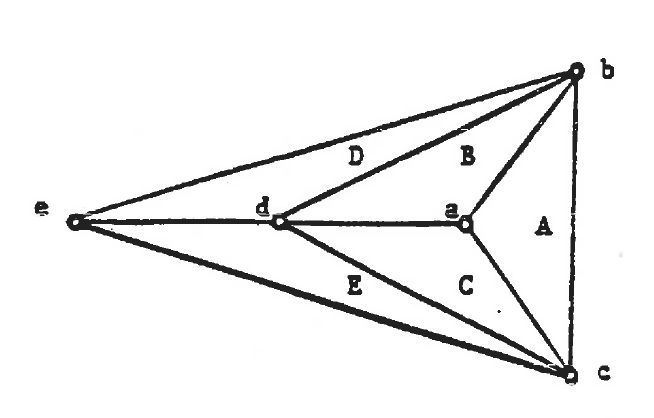
\includegraphics[width=.62\textwidth]{images/fig1.png}\par 图1\end{center}
\src{3}
设 $\Delta$ 为纯单纯复形。它的一个\textbf{壳序}是刻面的线性次序，使每个刻面与此前刻面生成的复形的交，是其若干极大真面的非空并。换言之，刻面的线性次序 $F_1,\ldots,F_t$ 是壳序，当且仅当
\[\begin{gathered}
\text{对每对 }F_i,F_j\ (1\le i<j\le t),\text{存在 }F_k\ (1\le k<j)\text{ 及 }x\in F_j,\\
F_i\cap F_j\subseteq F_k\cap F_j=F_j-x.
\end{gathered}\tag{7.3}\]
纯复形若有壳序，称为\textbf{可壳}的。每个零维复形都可壳；一维复形（简单图）可壳当且仅当连通。壳序的直观含义是：逐次加入刻面来构造纯 $d$ 维复形，每次把新刻面很好地贴到已构造部分上，使交在拓扑上是 $(d-1)$ 维球或 $(d-1)$ 维球面。
图1中，先将 $A,B,C$ 任意排列，再将 $D,E,F$ 任意排列，便得到壳序；但以 $A,B,E,\ldots$ 或 $D,E,C,A,\ldots$ 开始的次序不是壳序。
本节余下部分固定以下记号：$\Delta$ 是 $(r-1)$ 维可壳复形，$F_1,\ldots,F_t$ 按壳序排列。令 $\Delta_i=\{G\in\Delta:G\subseteq F_k\text{ 对某个 }k\le i\}$，即前 $i$ 个刻面生成的子复形。对 $i=1,\ldots,t$，令 $\RR(F_i)=\{x\in F_i:F_i-x\in\Delta_{i-1}\}$，称为壳序诱导的 $F_i$ 的\textbf{限制面}。于是 $\RR(F_i)=\varnothing$ 当且仅当 $i=1$；$\RR(F_i)=F_i$ 当且仅当其所有真子集都属于 $\Delta_{i-1}$。把 $\Delta$ 按面的包含关系排序，可在其中考虑布尔区间 $[G_1,G_2]=\{G:G_1\subseteq G\subseteq G_2\}$。
\st{命题7.2.2}区间 $[\RR(F_i),F_i]$（$i=1,\ldots,t$）划分可壳复形 $\Delta$。
\pr $F_1,\ldots,F_i$ 是 $\Delta_i$ 的壳序，故归纳地只需证明：(i) $\Delta_{t-1}\cup[\RR(F_t),F_t]=\Delta$；(ii) $\Delta_{t-1}\cap[\RR(F_t),F_t]=\varnothing$。若 $G\in\Delta-\Delta_{t-1}$，则 $G\subseteq F_t$。若某个 $x\in\RR(F_t)$ 不属于 $G$，则 $G\subseteq F_t-x\in\Delta_{t-1}$，矛盾。因此 $\RR(F_t)\subseteq G$，得到(i)。(ii)等价于 $\RR(F_t)\notin\Delta_{t-1}$。若不然，则对某个 $i<t$，$\RR(F_t)\subseteq F_i\cap F_t$。由(7.3)，存在 $k<t$ 及 $x\in F_t$，使 $\RR(F_t)\subseteq F_i\cap F_t\subseteq F_k\cap F_t=F_t-x$。
\src{4}
然而 $F_t-x\subseteq F_k\in\Delta_{t-1}$ 蕴含 $x\in\RR(F_t)$，与 $\RR(F_t)\subseteq F_t-x$ 矛盾。\qed
这表明：在壳化过程中把刻面 $F_i$ 及其子面加入 $\Delta_{i-1}$ 时，$\RR(F_i)$ 是 $F_i$ 中唯一极小的“新”面，即属于 $\Delta_i-\Delta_{i-1}$ 的极小面。定义可壳复形的\textbf{壳多项式}
\[h_\Delta(x)=\sum_{i=1}^t x^{|F_i-\RR(F_i)|}.\tag{7.4}\]
\st{命题7.2.3}若 $\Delta$ 可壳，则 $h_\Delta(1+\lambda)=f_\Delta(\lambda)$。因此壳多项式与壳序选择无关。
\pr 由二项式展开，
\[\begin{aligned}
h_\Delta(1+\lambda)&=\sum_i(1+\lambda)^{|F_i-\RR(F_i)|}\\
&=\sum_i\sum_{k=0}^r\binom{|F_i-\RR(F_i)|}{k}\lambda^k
=\sum_{k=0}^r\left(\sum_i\binom{|F_i-\RR(F_i)|}{k}\right)\lambda^k.
\end{aligned}\]
由命题7.2.2，$f_{r-k}=\sum_i\binom{|F_i-\RR(F_i)|}{k}$。\qed
所以 $h_\Delta(1)$ 等于刻面数，$h_\Delta(2)$ 等于总面数。更重要的是 $h_\Delta(0)=f_\Delta(-1)=(-1)^{r-1}\chi(\Delta)$。另一方面，由定义它等于满足 $\RR(F)=F$ 的刻面数。因此：
\st{推论7.2.4}$(-1)^{r-1}\chi(\Delta)$ 等于满足 $\RR(F)=F$ 的刻面 $F$ 的个数。\qed
取例7.2.1中的壳序 $A,B,C,D,E,F$，有 $\RR(A)=\varnothing$、$\RR(B)=\{d\}$、$\RR(C)=\{c,d\}$、$\RR(D)=\{e\}$、$\RR(E)=\{c,e\}$、$\RR(F)=F$。故
\[h_\Delta(x)=x^3+x^2+x+x^2+x+1=x^3+2x^2+2x+1.\]
可检验 $h_\Delta(2)=21$ 是总面数，$h_\Delta(1)=6$ 是刻面数，$h_\Delta(0)=1$ 等于欧拉示性数；而 $h_\Delta(1+\lambda)=\lambda^3+5\lambda^2+9\lambda+6=f_\Delta(\lambda)$。
写 $f_\Delta(\lambda)=\sum_{i=0}^rf_i\lambda^{r-i}$，$h_\Delta(x)=\sum_{i=0}^rh_ix^{r-i}$。称 $(f_0,\ldots,f_r)$ 和 $(h_0,\ldots,h_r)$ 分别为 $f$ 向量和 $h$ 向量。它们密切相关。比较 $f_\Delta(\lambda)=h_\Delta(1+\lambda)$ 的系数，得到
\[f_k=\sum_{i=0}^rh_i\binom{r-i}{k-i},\qquad k=0,\ldots,r.\tag{7.5}\]
\src{5}
类似地，由 $h_\Delta(x)=f_\Delta(x-1)$ 得逆公式
\[h_k=\sum_{i=0}^r(-1)^{i+k}f_i\binom{r-i}{k-i},\qquad k=0,\ldots,r.\tag{7.6}\]
因此 $h_0=f_0=1$，$h_1=f_1-r$。这也可直接由(7.4)得到，其等价表述为
\[h_k=\#\{\text{刻面 }F:|\RR(F)|=k\},\qquad0\le k\le r.\tag{7.7}\]
故所有 $h_k\ge0$。下面用 $f$ 向量与 $h$ 向量的关系研究可壳复形的若干计数事实，它们仅用于第7.5节。
\st{命题7.2.5}设 $\Delta$ 是顶点集 $V$ 上的 $(r-1)$ 维可壳复形，$|V|=v>r$。则：
\begin{enumerate}[label=(\roman*)]
\item 对所有 $0\le k<j\le r-k$，有 $f_k<f_j$。
\item 若 $1\le k<(r+1)/2$ 且 $h_{r-k+1}\ge1$，则 $f_k\le f_{r-k+1}$；等号成立当且仅当还满足 $h_2=1$。
\item 若 $V$ 的所有 $e$ 元子集均属于 $\Delta$，其中 $e<r$，则
\[f_k\ge\sum_{i=0}^e\binom{v-r+i-1}{i}\binom{r-i}{k-i},\qquad k=0,\ldots,r.\]
而且下列条件等价：$(\alpha)$ 对某个 $k>e$ 等号成立；$(\beta)$ 对所有 $k$ 等号成立；$(\gamma)$ $f_r=\binom{v-r+e}{e}$。
\end{enumerate}
\pr (i)直接由(7.5)、(7.7)中的非负性和二项式系数的初等性质得到。(ii)需要进一步使用 $h$ 向量的结构，见习题7.2.2。
对(iii)，假设所有 $e$ 元子集都是面，即 $f_k=\binom vk$（$k=0,\ldots,e$）。用恒等式 $(-1)^y\binom{-x}{y}=\binom{x+y-1}{y}$ 和 Vandermonde 卷积 $\binom{x+y}k=\sum_i\binom xi\binom y{k-i}$，由(7.6)，对 $k\le e$ 得
\[\begin{aligned}
h_k&=\sum_{i=0}^k(-1)^{i+k}\binom{r-i}{k-i}\binom vi\\
&=\sum_{i=0}^k\binom{k-r-1}{k-i}\binom vi=\binom{v-r+k-1}k.
\end{aligned}\tag{7.8}\]
代入(7.5)，并用 $k>e$ 时的 $h_k\ge0$，保留前 $e+1$ 项即得不等式。同一论证说明，若 $(\delta)$ $h_{e+1}=\cdots=h_r=0$，则所有 $k$ 都取等。因此 $(\delta)\Rightarrow(\beta)\Rightarrow(\gamma)\Rightarrow(\alpha)$，其中$(\gamma)$就是 $k=r$ 时取等。若某个 $k>e$ 取等，(7.5)给出 $h_{e+1}=\cdots=h_k=0$。
\src{6}
由下述引理结合(7.7)，其后的 $h_{k+1},\ldots,h_r$ 也均为零，故 $(\alpha)\Rightarrow(\delta)$。\qed
\st{引理7.2.6}设 $\mathcal F=\{\RR(F_i):1\le i\le t\}$，其中 $F_1,\ldots,F_t$ 是 $\Delta$ 的壳序。则对任意 $A\in\mathcal F-\{\varnothing\}$，存在 $x\in A$ 使 $A-x\in\mathcal F$。
\pr 设 $1<g\le t$，令 $X_1,\ldots,X_s$ 是 $\RR(F_g)$ 的极大真子集。由于 $\RR(F_g)$ 是 $\Delta_g-\Delta_{g-1}$ 中唯一极小面，它们都属于 $\Delta_{g-1}$。由命题7.2.2，存在唯一的刻面 $F_{i_j}$，使 $\RR(F_{i_j})\subseteq X_j\subseteq F_{i_j}$ 且 $i_j<g$。不同 $j,k$ 对应不同刻面；否则 $\RR(F_g)=X_j\cup X_k\subseteq F_{i_j}$，与命题7.2.2矛盾。不妨 $i_1<\cdots<i_s$。$X_s$ 的每个真子集都属于 $\Delta_{i_s-1}$，故 $\RR(F_{i_s})$ 不可能真包含于 $X_s$。因此 $\RR(F_{i_s})=X_s\subset\RR(F_g)$，且 $|\RR(F_g)|=|\RR(F_{i_s})|+1$。\qed
